\documentclass[11pt]{article}
\usepackage[UTF8]{ctex}
\usepackage[a4paper]{geometry}
\geometry{left=2.0cm,right=2.0cm,top=2.5cm,bottom=2.5cm}

\usepackage{comment}
\usepackage{booktabs}
\usepackage{graphicx}
\usepackage{diagbox}
\usepackage{amsmath,amsfonts,graphicx,amssymb,bm,amsthm}
\usepackage{algorithm,algorithmicx}
\usepackage[noend]{algpseudocode}
\usepackage{fancyhdr}
\usepackage{tikz}
\usepackage{graphicx}
\usepackage{verbatim}
\usetikzlibrary{arrows,automata}
\usepackage{hyperref}
\usepackage{listings}

\setlength{\headheight}{14pt}
\setlength{\parindent}{0 in}

\newtheorem{theorem}{Theorem}
\newtheorem{lemma}[theorem]{Lemma}
\newtheorem{proposition}[theorem]{Proposition}
\newtheorem{claim}[theorem]{Claim}
\newtheorem{corollary}[theorem]{Corollary}
\newtheorem{definition}[theorem]{Definition}


\newcommand\E{\mathbb{E}}
\newcommand{\labid}{1}			% 第几次作业
\newcommand{\name}{Yuyang Zhou} 		% 你的名字
\newcommand{\id}{2000013061} 	% 你的学号


\usetikzlibrary{positioning}

\begin{document}

    \pagestyle{fancy}
    \lhead{Peking University}
    \chead{}
    \rhead{CompNet}

    \begin{center}
        {\LARGE \bf README for LAB \#\labid}\\
        {\Large \name}\\
        {\Large \id}\\
    \end{center}

	\section{Implemented}
		\par The features implemented are \texttt{PT1, PT2}. and this document include the answer of \texttt{WT1}
		
	\section{WT1}
	
		\par 1. there are 827 frame in total
		\par 2. ff:ff:ff:ff:ff:ff
		
		The destination address is special because it is a boardcast message. 
		The computer with MAC address 6a:15:0a:ba:9b:7c doesn't know which computer have IP address 10.0.0.88/10.0.0.24, and it boardcast the message to all computers, trying to find the one with IP address 10.0.0.88/10.0.0.24.
		\par 3. 0x15 in hexademical, 21 in demical 
		
		
	\section{Code Arrangement}
	
	\subsection*{macro.h}
		\par define the macros used in the following programs.
		
	\subsection*{constant.h}
		\par define the constants used in the following programs.
		
	\subsection*{type.h}
		\par define the specific types used in the following programs.
		
	\subsection*{name2mac.h}
		\par find the Mac Address(actually hardware address) of specific device
	\begin{itemize}
		\item \texttt{findMac(const char* device, uint8\_t* mac\_addr)}
		
		* find the Mac Address of specific device
		
		* @param device the name of the device request for Mac address
		
		* @param mac\_addr the pointer to the memory used to save the
		Mac address
		
		* @return 0 on success, 1 on failure.
	\end{itemize}
	
		
	\subsection*{device.h}
		\par Library supporting network device management.
		\begin{itemize}
			\item \texttt{checkDevice(const char* device)}
			
			* Check whether the device name exists in the network.
			
			* @param device Name of network device to check.
			
			* @return True on success , False on error.
			
			
			\item \texttt{addDevice(const char* device)}
			
			* Add a device to the library for sending / receiving packets .
			
			* @param device Name of network device to send / receive packet on .
			
			* @return A non - negative \_device - ID\_ on success , -1 on error .
			
			\item \texttt{findDevice(const char* device)}
			
			* Find a device added by 'addDevice'.
			
			* @param device Name of the network device .
			
			* @return A non - negative \_device - ID\_ on success , -1 if no such device was found .
		\end{itemize}
		
		In order to manage this, the code two structures \texttt{DeviceNode} and \texttt{DeviceManager}, and implements the following methods
		
		\begin{itemize}
			\item \texttt{DeviceNode}
			
			\begin{itemize}
				\item \texttt{char* device\_names} The name of the device 
				\item \texttt{pcap\_t* receive\_handler} The handler used to receive messages
				\item \texttt{pcap\_t* send\_handler} The handler used to send messages
				\item \texttt{frameReceiveCallback callback} The default callback function
				\item \texttt{uint8\_t mac\_addr[8]} Mac address of the device
				\item \texttt{int index} The index of the device
				\item \texttt{bool isEqualDevice(const char* device)}
				
				* Check if the name of the device is equal to 'device'
				
				* @param device The name of device to check out
				
				* @return True on same, False on different
				
				\item \texttt{void setCallback(frameReceiveCallback \_\_callback\_\_)}
				
				* Set up the callback function of the device
				
				* @param \_\_callback\_\_ the pointer of callback function to set up
				
				\item \texttt{int setDevice(const char* device)}
					
				* Initalize the deviceNode with name device
				
				* @param device The name of device used to set up
				
				* @return 0 on success, -1 on failure. 
				
				\item \texttt{int handInPacket(struct pcap\_pkthdr* pkt\_header, const u\_char* framebuf)}
				
				* Handle the infomation of the package founc by libpcap
				
				* @param pkt\_header the header of the packet found
				
				* @param framebuf the information of the packet found
				
				* @return 0 on success, -1 on failure. 
				
			\end{itemize}
			
			\item \texttt{DeviceManager}
			
			\begin{itemize}
				\item \texttt{DeviceNode** device\_list} The pointer to the piece of memory, to save the pointer of \texttt{DeviceNode}s
				\item \texttt{int device\_count} The number of devices in the manager
				\item \texttt{int device\_bound} The maximum number of devices can be saved now
				\item \texttt{DeviceNode* operator [](const int index)}
				
				* Return the pointer of the index-th DeviceNode
				
				* @param index The index of device to find
				
				\item \texttt{int addDevice(const char* device)}
				
				* Add a device to the library for sending / receiving packets .
				
				* @param device Name of network device to send / receive packet on .
				
				* @return A non - negative \_device - ID\_ on success , -1 on error .
				
				\item \texttt{findDevice(const char* device)}
				
				* Find a device added by 'addDevice'.
				
				* @param device Name of the network device .
				
				* @return A non - negative \_device - ID\_ on success , -1 if no such device was found .
				
				\item \texttt{count()}
				
				* @return The number of devices in the manager.
			\end{itemize}
		\end{itemize}
	
	
	\subsection*{packetio.h}
	\par Library supporting sending / receiving Ethernet II frames.
	\begin{itemize}
		\item \texttt{int sendFrame (const void * buf, int len, int ethtype, const void *destmac, int id)}
		
		* Encapsulate some data into an Ethernet II frame and send it .
		
		* @param buf Pointer to the payload .
		
		* @param len Length of the payload .
		
		* @param ethtype EtherType field value of this frame .
		
		* @param destmac MAC address of the destination .
		
		* @param id ID of the device ( returned by "addDevice") to send on .
		
		* @return 0 on success , -1 on error .
		
		\item \texttt{int setFrameReceiveCallback(frameReceiveCallback callback, int id)}
		
		* Register a callback function to be called each time an Ethernet II frame was received .
		
		*@param callback the callback function.
		
		* @return 0 on success , -1 on error.
		
		\item \texttt{int receiveAllFrame(int id, int frame\_count)}
		
		* try to receive specific number of Ethernet frames from device ID id.
		
		* @param id The Index of device to receive the package.
		
		* @param frame\_count A number,-1 represents receiving until error occurs, 0-65535 represents the number of packet expected to receive.
		
		* @return the number of packages received,
	\end{itemize}
	
	\subsection*{main.cpp}
		
	\begin{itemize}
		\item \texttt{msg} test message to send.
		
		\item \texttt{egCallback(const void* \_\_buffer, const void* \_\_mac\_addr, int len, int index))}
		
		* Example Callback function.
		
		* @param \_\_buffer the message from the packet.
		
		* @param \_\_mac\_addr the mac address of the source of the packet.
		
		* @param len the length of \_\_buffer
		
		* @param the index of device which receive the packet.
		
		* @return 0 on success, 1 on failure.
	\end{itemize}
		
		
		
	\section{Implementing Details}
	
	\subsection*{name2mac.h}
	
	\par The piece of code use \texttt{socket} and \texttt{ioctl} to find the MAC address, instead of directly reading files from \texttt{/etc/ether}. 
	
	\par And because of that, the code require root access to run, otherwise it will fail to find the MAC address.
	
	\subsection*{device.h}
	
	\par This piece of code use structure \texttt{DeviceNodes} to maintain all informations about specific devices, and this may helps to reduce the difficulty of the following labs. And also, each \texttt{DeviceNodes} use two different handlers, one for sending packets, and the other one for receiving packets. The receiver use a filter, so that it only react the packet which the destination address is the same as the mac address of the device. Also, there may have different callback function for different devices, so I choose to save the function for each device.
	
	\par \texttt{DeviceManager} maintain a list, which save the pointer of all \texttt{DeviceNodes}. I use a hand-written memory management instead of directly \texttt{vector<DeviceNode>}, because the copy of \texttt{DeviceNode} may cause serious memory leaking. So I copy the pointer, instead of copy the structure itself.
	
	\par In addition, \texttt{checkDevice} gives a interface, which can check that whether the specific device exists. And It will fail to add a device, if the manager could not find it.
	
	\subsection*{packetio.h}
	
	\par Because we have find the MAC address of the device, we can simply splicing all information we have to obtain the raw Ethernet frame. And the frame could be send through the \texttt{send-handler} we have create in \texttt{addDevice}.
	
	\par In \text{receiveAllFrame}, Because we have set the filter \texttt{'ether dst xx:xx:xx:xx:xx:xx'}, we can find and only find the frame which is send to the specific device. The \texttt{frame\_count} parameter, like \texttt{pcap\_loop}, is designed for further labs. And because we have set non-blocking for the receiving handler, we must return the number of frame we have received due to delays.
	
	\subsection*{main.cpp}
	
	\par This part gives a example \texttt{egCallback()} function, which helps me to check whether the packets received are correctly handled.
	
	\par The main function firstly print the name, and discription about all devices in the ethernet, and the MAC address of the devices if exists. Then it will insert all devices with MAC address into the device manager. After that it will try to send a raw Ethernet frame from device $0$ to device $0$, where device $0$, the first device we insert, may be \texttt{ens33}(In my conputer) or \texttt{eth0}(Other computers). At last, it will catch $5$ frames to device $0$, and call \texttt{egCallBack()} $5$ times, which print the information about the frame.
	
	\section{Usage}
	
	The executable file is generated using \texttt{cmake}.
	
	\lstset{language = bash}
	\begin{lstlisting}
		mkdir build && cd build
		cmake ..
		make
	\end{lstlisting}
	
	Then executable file is saved in \texttt{/build/src/lab1}, and you can use the following command to run it.
	
	\begin{lstlisting}
	sudo ./src/lab1
	\end{lstlisting}

	\section{CheckPoint}
	
	\subsection*{CP1}
	
	The following image shows that we try to send a message \texttt{msg} which is defined in \texttt{main.cpp}. After senging out the message, the packet is catched by wireshark, and the frame if sent correctly.
	
	\begin{figure}[htbp]
	\centering
	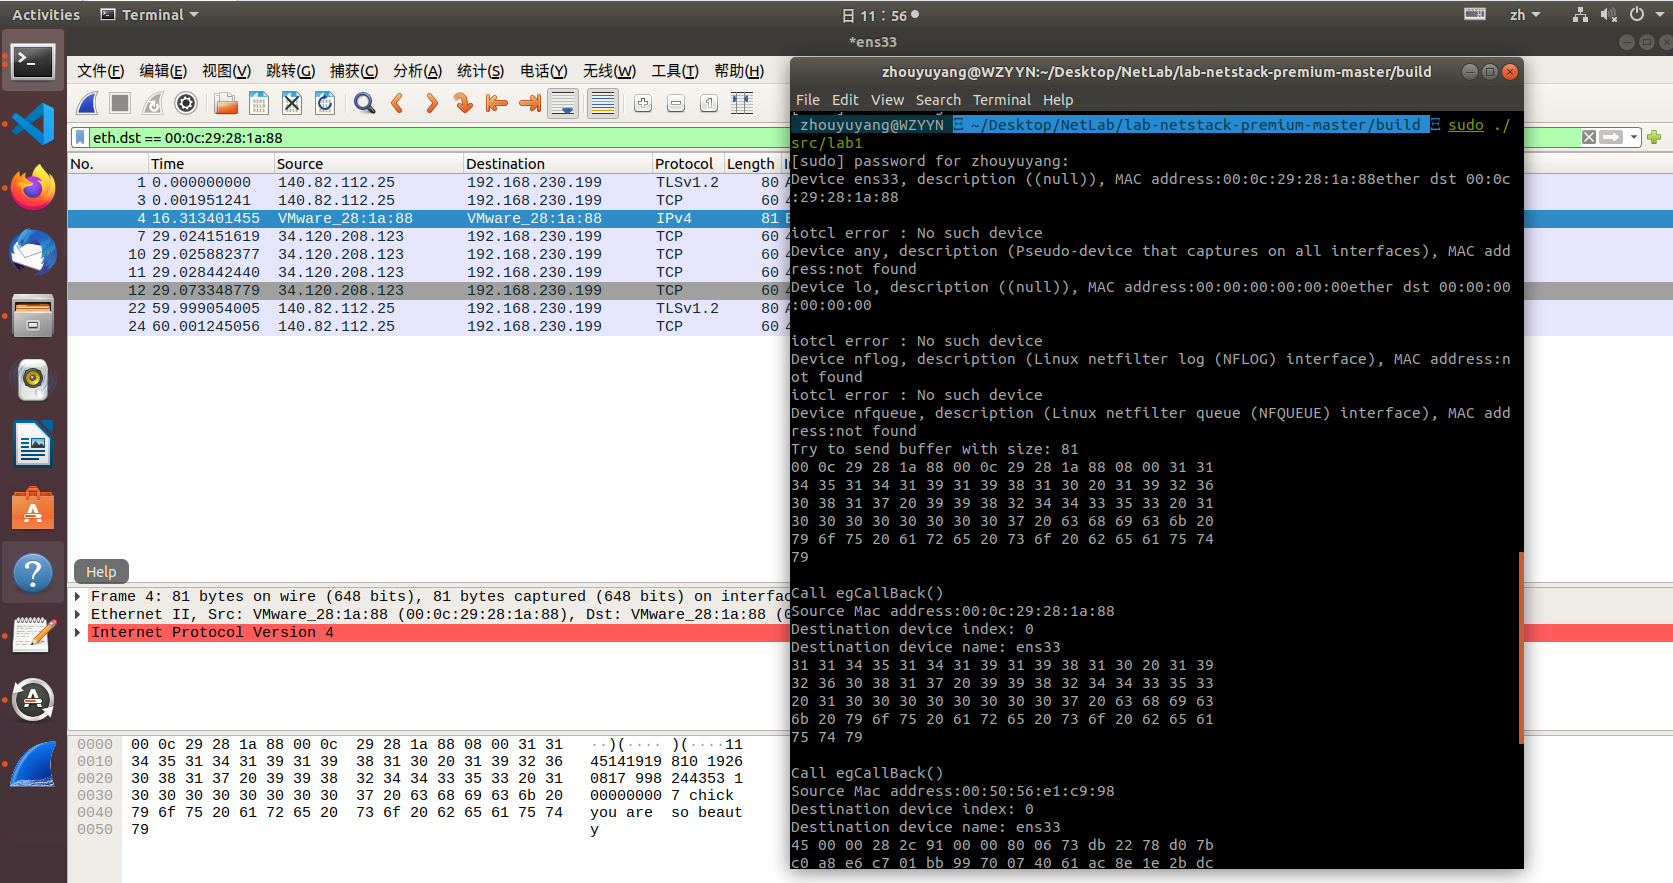
\includegraphics[width=0.65\linewidth]{../lab-netstack-premium-master/checkpoints/CP1.png}
	\caption{CP-1: The program send a frame, and it is catched by wireshark}
	\label{fig:CP1}
	\end{figure}
	
	\subsection*{CP2}
	
	The following image shows that the frame we send is successfully to \texttt{egCallBack()}
	
	\begin{figure}[htbp]
		\centering
		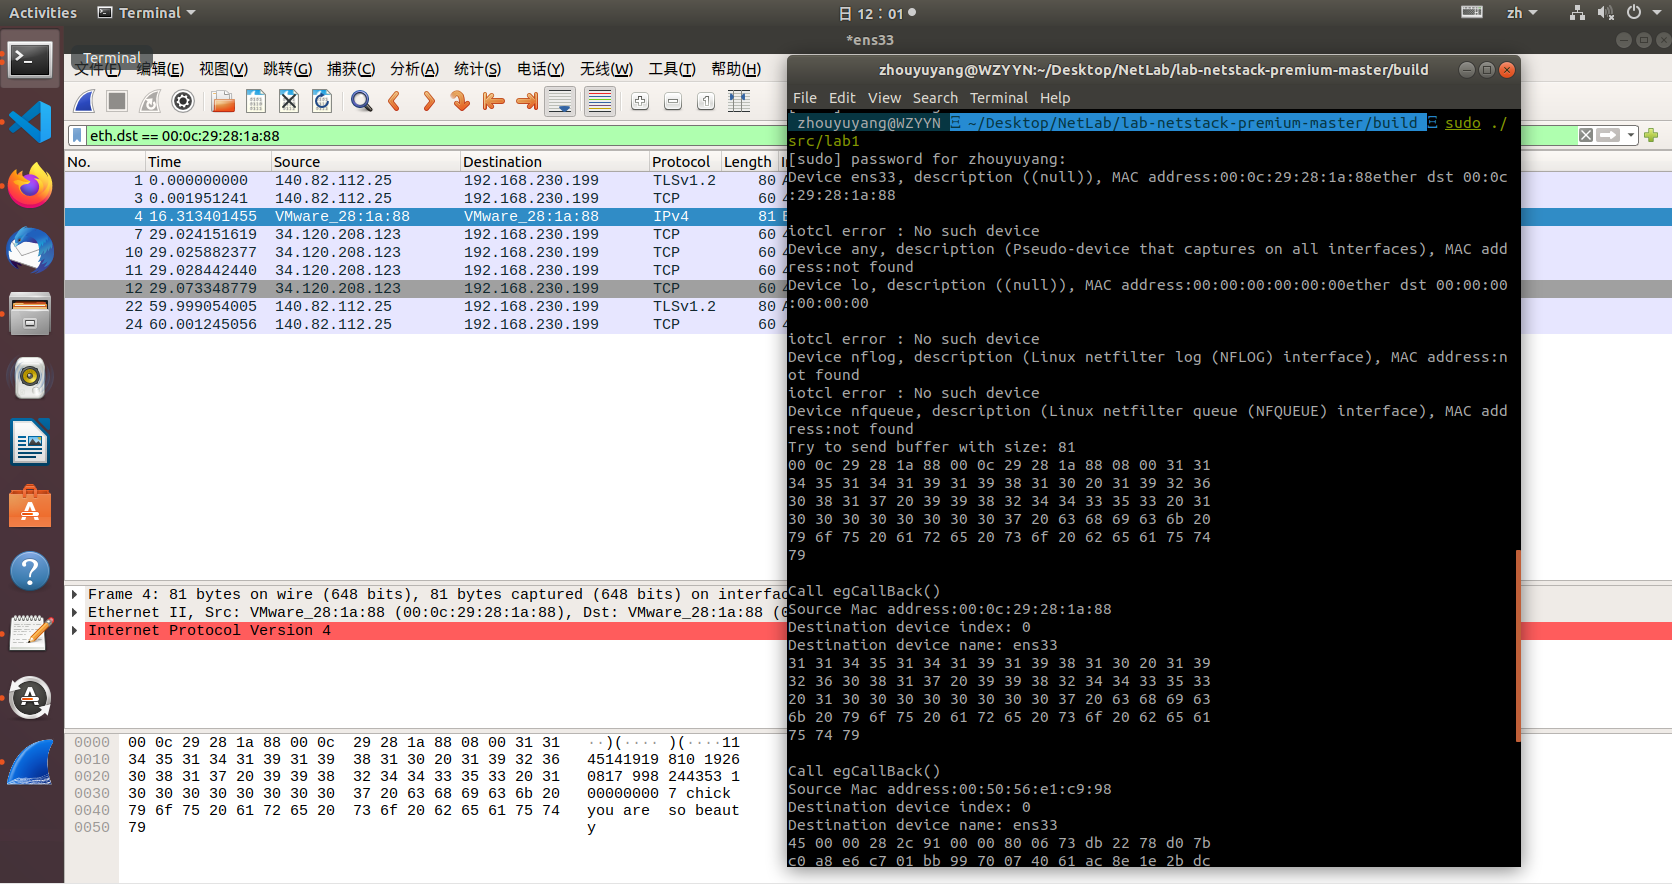
\includegraphics[width=0.65\linewidth]{../lab-netstack-premium-master/checkpoints/CP2-1.png}
		\caption{CP2-1: The program receive the frame we send}
		\label{fig:CP2-1}
	\end{figure}
	
	The following image shows that the fifth frame we catch is exactly the fifth frame which is send to the device.
	
	\begin{figure}[htbp]
		\centering
		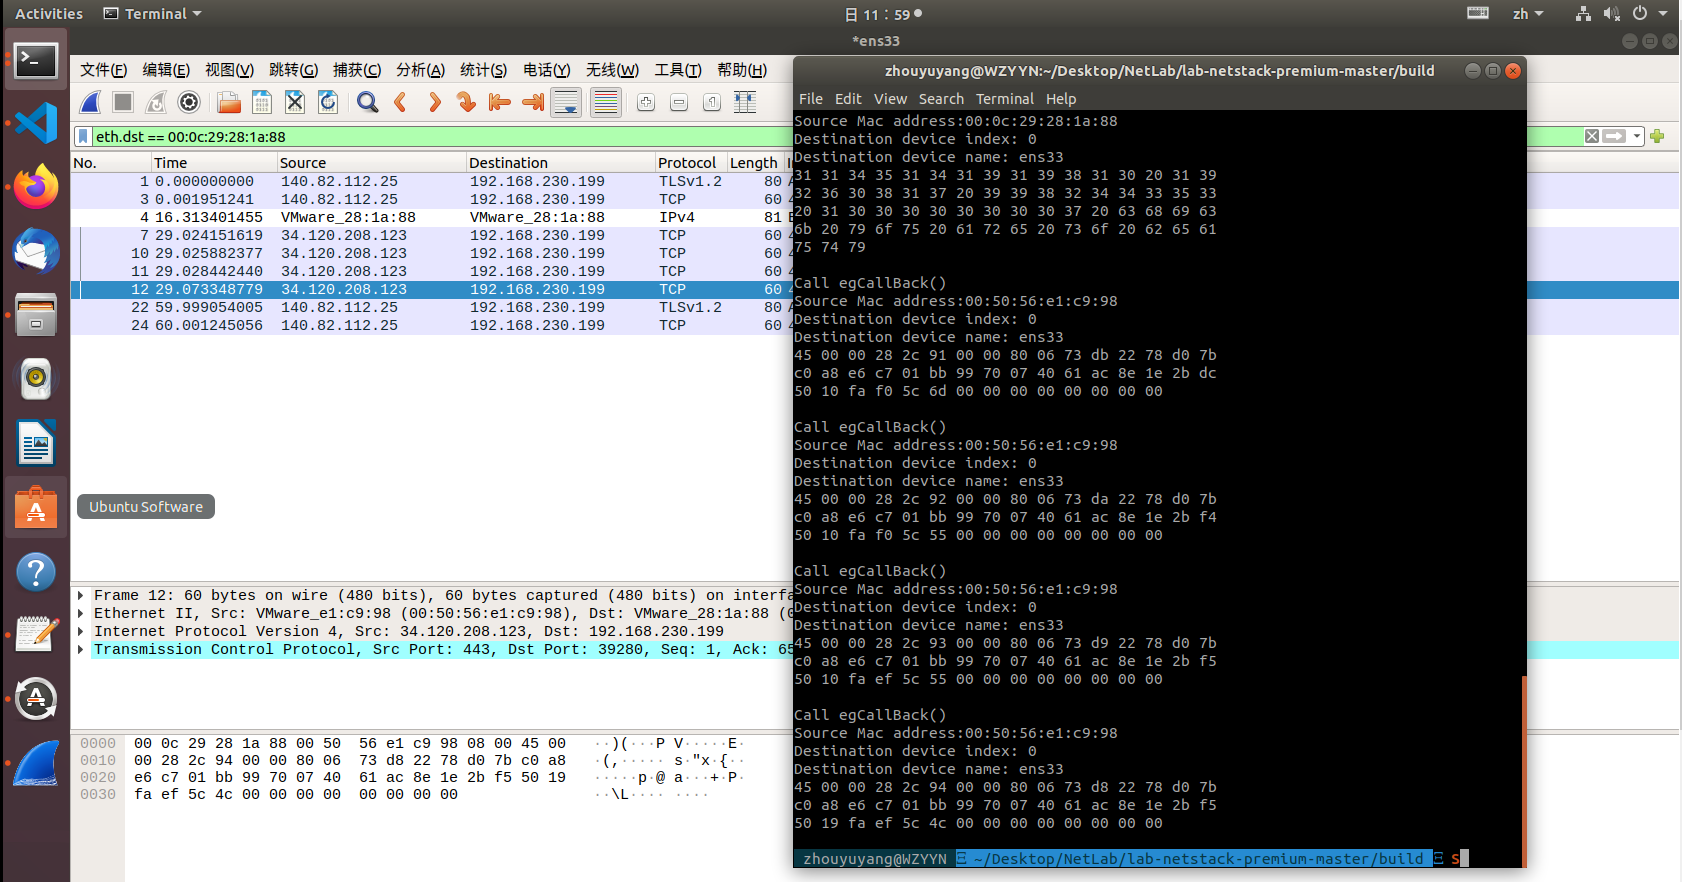
\includegraphics[width=0.65\linewidth]{../lab-netstack-premium-master/checkpoints/CP2-2.png}
		\caption{CP2-2: The fifth frame we receive}
		\label{fig:CP2-2}
	\end{figure}
	
	All these pictures can be found in \texttt{/checkpoints}.
		
\end{document}